
\subsection{基于图片信息的无监督神经机器翻译}
\begin{figure}[!htbp]
    \centering
    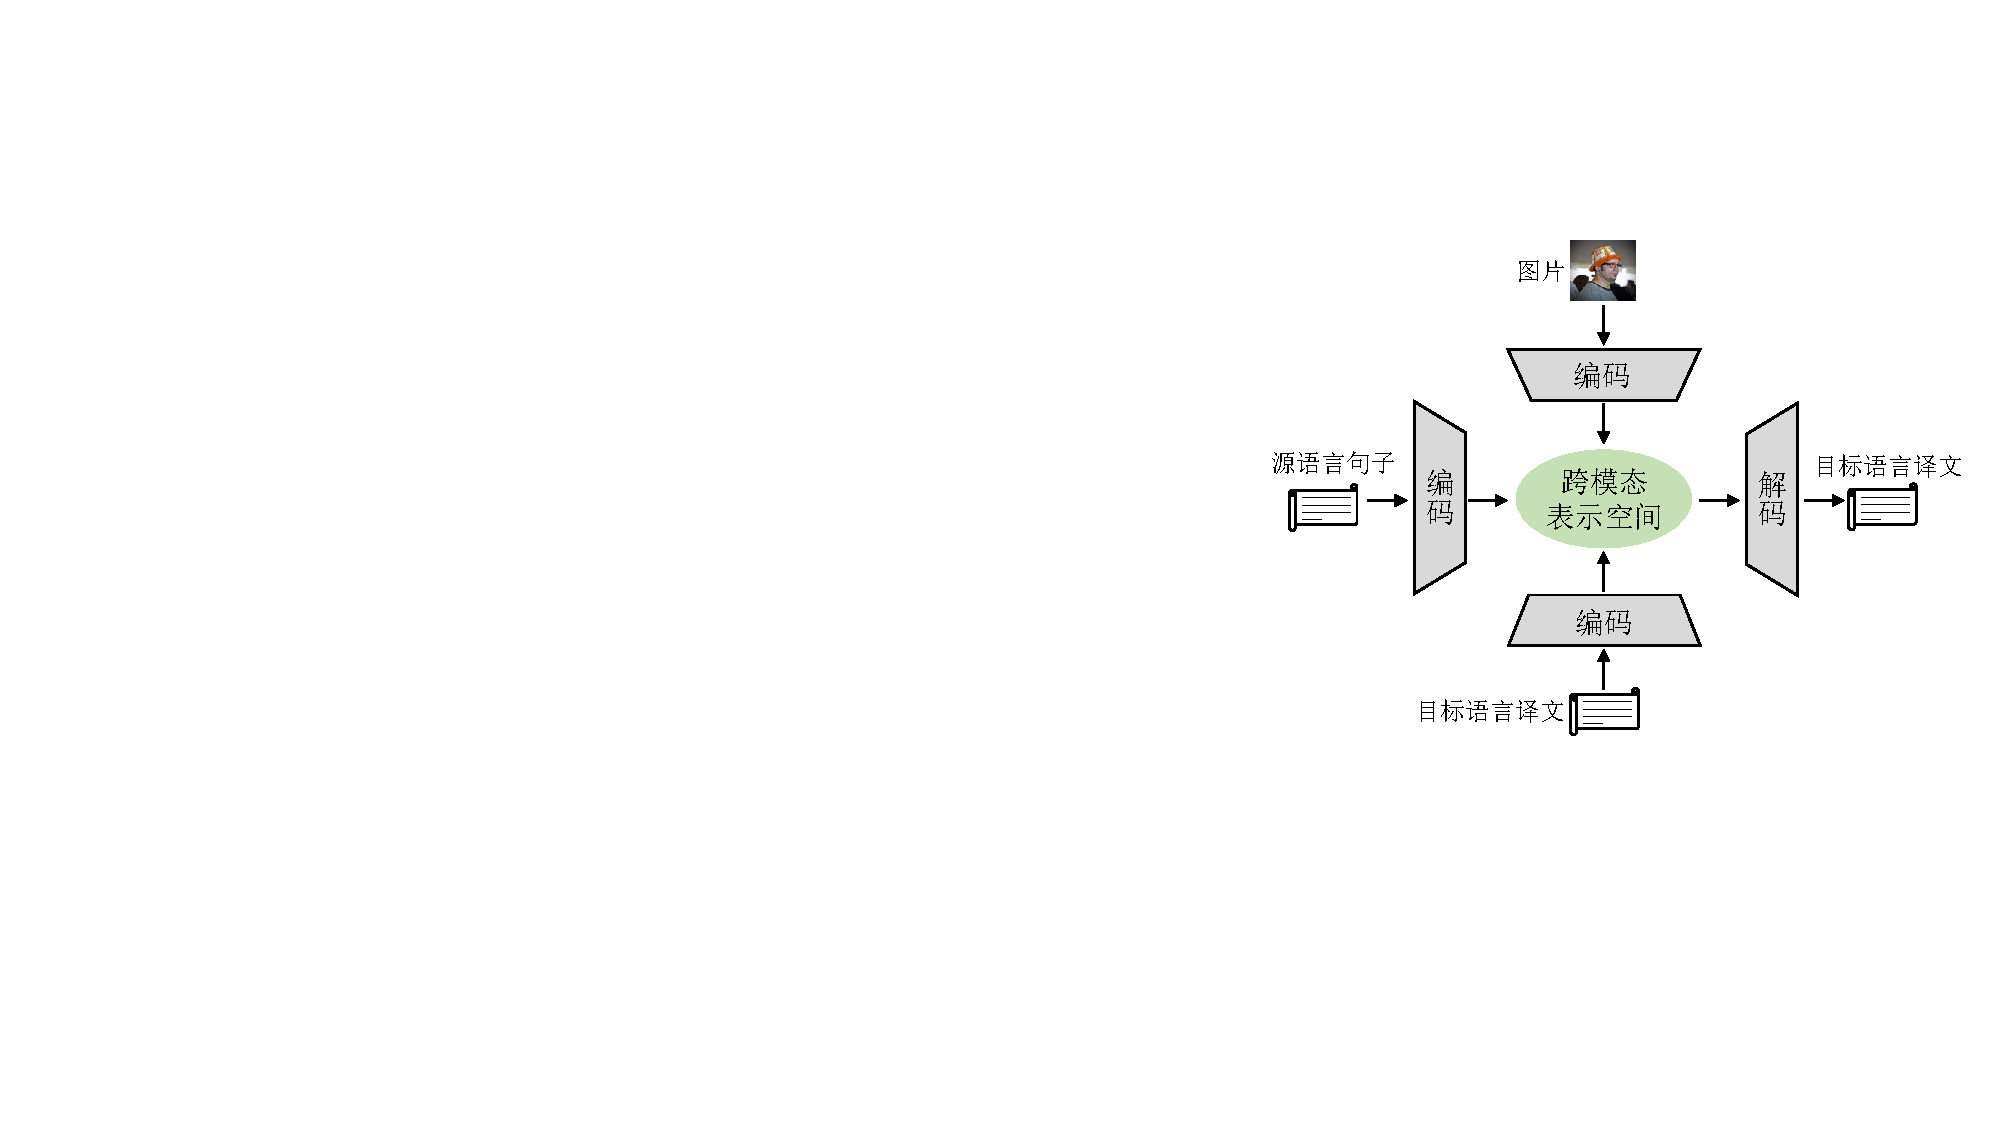
\includegraphics[scale=1]{Img/fig_2_iunmt.pdf}
    \bicaption{基于图片信息的无监督神经机器翻译}{Image-based unsupervised neural machine translation}
    \label{fig:2_iunmt}
\end{figure}
基于图片信息的无监督神经机器翻译(image-based unsupervised neural machine translation,IUNMT)是指利用图片作为语言桥梁,为零资源的翻译提供翻译支持的一类方法。零资源语言的翻译问题通常选择一个中间语言作为桥梁,通过将源语言翻译到中间语言,再将中间语言翻译到目标语言的方式,解决源语言到目标语言的翻译问题。然而,这种方法仍然需要源语言和目标语言到中间语言的平行翻译数据,而很多的低资源语言之间的翻译很难通过这种办法解决。考虑到人的语言可能分为多种,但人眼中的世界是统一的,并且社交媒体中包含了大量的单语的图文数据,所以选择视觉模态作为中间语言来完成零资源机器翻译任务是一个很好的选择。
\tcite{saha2016correlational}采用了中间语言方案解决源语言与目标语言之间没有平行的训练数据的问题。该方法选择图片作为中间语言,通过联合训练源语言到图片和图片到目标语言的生成模型,最终过得源语言到目标语言的翻译模型。
\tcite{nakayama2017zero}同样将图片作为了中间语言,在训练过程中,将源语言、目标语言、和图片映射到一个统一的跨模态表示空间。
\tcite{chen2018zeroresource}将零资源的神经机器翻译模型的训练过程构建为一个多智能体交流游戏(multi-agent communication game)。每个智能体分别负责从图片中生成描述,以及从描述中生成目标语言译文的任务。两个智能体在两种任务的配合下完成源语言到目标语言的翻译建模。
\tcite{su2019unsupervised}采用降噪模型的训练方式构建中间语言与源语言和目标语言的编码器和解码器,在联合使用编码器和解码器的情况下实现源语言到目标语言之间的翻译。
\tcite{chen2019from}认为图片中包含太多与待翻译句子以及译文不相关信息,直接作为句子级语义单位的中间语言会引入大量噪音,因此将图片先应用到词的翻译,在通过迭代生成伪平行句对的方式,逐步实现句子级的翻译。
\tcite{huang2020unsupervised}同样通过图片生成伪平行句对的方式逐步训练翻译模型。

